\documentclass[twoside]{book}

% Packages required by doxygen
\usepackage{fixltx2e}
\usepackage{calc}
\usepackage{doxygen}
\usepackage[export]{adjustbox} % also loads graphicx
\usepackage{graphicx}
\usepackage[utf8]{inputenc}
\usepackage{makeidx}
\usepackage{multicol}
\usepackage{multirow}
\PassOptionsToPackage{warn}{textcomp}
\usepackage{textcomp}
\usepackage[nointegrals]{wasysym}
\usepackage[table]{xcolor}

% Font selection
\usepackage[T1]{fontenc}
\usepackage[scaled=.90]{helvet}
\usepackage{courier}
\usepackage{amssymb}
\usepackage{sectsty}
\renewcommand{\familydefault}{\sfdefault}
\allsectionsfont{%
  \fontseries{bc}\selectfont%
  \color{darkgray}%
}
\renewcommand{\DoxyLabelFont}{%
  \fontseries{bc}\selectfont%
  \color{darkgray}%
}
\newcommand{\+}{\discretionary{\mbox{\scriptsize$\hookleftarrow$}}{}{}}

% Page & text layout
\usepackage{geometry}
\geometry{%
  a4paper,%
  top=2.5cm,%
  bottom=2.5cm,%
  left=2.5cm,%
  right=2.5cm%
}
\tolerance=750
\hfuzz=15pt
\hbadness=750
\setlength{\emergencystretch}{15pt}
\setlength{\parindent}{0cm}
\setlength{\parskip}{0.2cm}
\makeatletter
\renewcommand{\paragraph}{%
  \@startsection{paragraph}{4}{0ex}{-1.0ex}{1.0ex}{%
    \normalfont\normalsize\bfseries\SS@parafont%
  }%
}
\renewcommand{\subparagraph}{%
  \@startsection{subparagraph}{5}{0ex}{-1.0ex}{1.0ex}{%
    \normalfont\normalsize\bfseries\SS@subparafont%
  }%
}
\makeatother

% Headers & footers
\usepackage{fancyhdr}
\pagestyle{fancyplain}
\fancyhead[LE]{\fancyplain{}{\bfseries\thepage}}
\fancyhead[CE]{\fancyplain{}{}}
\fancyhead[RE]{\fancyplain{}{\bfseries\leftmark}}
\fancyhead[LO]{\fancyplain{}{\bfseries\rightmark}}
\fancyhead[CO]{\fancyplain{}{}}
\fancyhead[RO]{\fancyplain{}{\bfseries\thepage}}
\fancyfoot[LE]{\fancyplain{}{}}
\fancyfoot[CE]{\fancyplain{}{}}
\fancyfoot[RE]{\fancyplain{}{\bfseries\scriptsize Generated on Tue Oct 13 2015 16\+:15\+:57 for My Project by Doxygen }}
\fancyfoot[LO]{\fancyplain{}{\bfseries\scriptsize Generated on Tue Oct 13 2015 16\+:15\+:57 for My Project by Doxygen }}
\fancyfoot[CO]{\fancyplain{}{}}
\fancyfoot[RO]{\fancyplain{}{}}
\renewcommand{\footrulewidth}{0.4pt}
\renewcommand{\chaptermark}[1]{%
  \markboth{#1}{}%
}
\renewcommand{\sectionmark}[1]{%
  \markright{\thesection\ #1}%
}

% Indices & bibliography
\usepackage{natbib}
\usepackage[titles]{tocloft}
\setcounter{tocdepth}{3}
\setcounter{secnumdepth}{5}
\makeindex

% Hyperlinks (required, but should be loaded last)
\usepackage{ifpdf}
\ifpdf
  \usepackage[pdftex,pagebackref=true]{hyperref}
\else
  \usepackage[ps2pdf,pagebackref=true]{hyperref}
\fi
\hypersetup{%
  colorlinks=true,%
  linkcolor=blue,%
  citecolor=blue,%
  unicode%
}

% Custom commands
\newcommand{\clearemptydoublepage}{%
  \newpage{\pagestyle{empty}\cleardoublepage}%
}

\usepackage{caption}
\captionsetup{labelsep=space,justification=centering,font={bf},singlelinecheck=off,skip=4pt,position=top}

%===== C O N T E N T S =====

\begin{document}

% Titlepage & ToC
\hypersetup{pageanchor=false,
             bookmarks=true,
             bookmarksnumbered=true,
             pdfencoding=unicode
            }
\pagenumbering{roman}
\begin{titlepage}
\vspace*{7cm}
\begin{center}%
{\Large My Project }\\
\vspace*{1cm}
{\large Generated by Doxygen 1.8.11}\\
\vspace*{0.5cm}
{\small Tue Oct 13 2015 16:15:57}\\
\end{center}
\end{titlepage}
\clearemptydoublepage
\tableofcontents
\clearemptydoublepage
\pagenumbering{arabic}
\hypersetup{pageanchor=true}

%--- Begin generated contents ---
\chapter{File Index}
\section{File List}
Here is a list of all files with brief descriptions\+:\begin{DoxyCompactList}
\item\contentsline{section}{\hyperlink{test_8c}{test.\+c} }{\pageref{test_8c}}{}
\end{DoxyCompactList}

\chapter{File Documentation}
\hypertarget{test_8c}{}\section{test.\+c File Reference}
\label{test_8c}\index{test.\+c@{test.\+c}}
{\ttfamily \#include $<$assert.\+h$>$}\\*
{\ttfamily \#include $<$unistd.\+h$>$}\\*
{\ttfamily \#include $<$string.\+h$>$}\\*
{\ttfamily \#include $<$pthread.\+h$>$}\\*
{\ttfamily \#include $<$stdio.\+h$>$}\\*
{\ttfamily \#include $<$nanomsg/nn.\+h$>$}\\*
{\ttfamily \#include $<$nanomsg/pipeline.\+h$>$}\\*
Include dependency graph for test.\+c\+:
\nopagebreak
\begin{figure}[H]
\begin{center}
\leavevmode
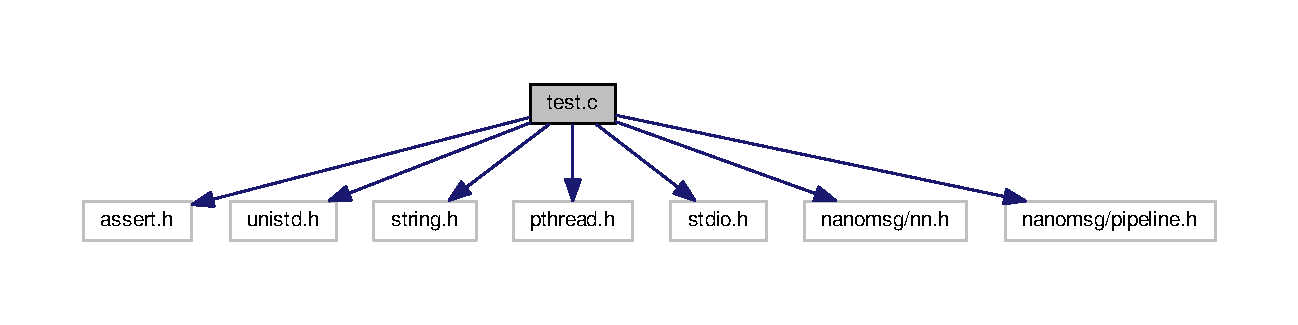
\includegraphics[width=350pt]{test_8c__incl}
\end{center}
\end{figure}
\subsection*{Macros}
\begin{DoxyCompactItemize}
\item 
\#define \hyperlink{test_8c_a944b91dfe8c77b9676151af5e1acfc07}{N\+O\+D\+E0}~\char`\"{}node0\char`\"{}
\item 
\#define \hyperlink{test_8c_a0083b501f8bcda9622f407e919c23901}{N\+O\+D\+E1}~\char`\"{}node1\char`\"{}
\end{DoxyCompactItemize}
\subsection*{Functions}
\begin{DoxyCompactItemize}
\item 
int \hyperlink{test_8c_a084294b3519ee89229dea2e629b62bc1}{node0} (const char $\ast$url)
\item 
int \hyperlink{test_8c_aea33b29a6a2a2006cc876dbb26586c71}{node1} (const char $\ast$url, const char $\ast$msg)
\item 
int \hyperlink{test_8c_ac762d48b889bd832ec0d42abcbc50624}{main} (const int argc, const char $\ast$$\ast$argv)
\end{DoxyCompactItemize}


\subsection{Macro Definition Documentation}
\index{test.\+c@{test.\+c}!N\+O\+D\+E0@{N\+O\+D\+E0}}
\index{N\+O\+D\+E0@{N\+O\+D\+E0}!test.\+c@{test.\+c}}
\subsubsection[{N\+O\+D\+E0}]{\setlength{\rightskip}{0pt plus 5cm}\#define N\+O\+D\+E0~\char`\"{}node0\char`\"{}}\hypertarget{test_8c_a944b91dfe8c77b9676151af5e1acfc07}{}\label{test_8c_a944b91dfe8c77b9676151af5e1acfc07}
\index{test.\+c@{test.\+c}!N\+O\+D\+E1@{N\+O\+D\+E1}}
\index{N\+O\+D\+E1@{N\+O\+D\+E1}!test.\+c@{test.\+c}}
\subsubsection[{N\+O\+D\+E1}]{\setlength{\rightskip}{0pt plus 5cm}\#define N\+O\+D\+E1~\char`\"{}node1\char`\"{}}\hypertarget{test_8c_a0083b501f8bcda9622f407e919c23901}{}\label{test_8c_a0083b501f8bcda9622f407e919c23901}


\subsection{Function Documentation}
\index{test.\+c@{test.\+c}!main@{main}}
\index{main@{main}!test.\+c@{test.\+c}}
\subsubsection[{main(const int argc, const char $\ast$$\ast$argv)}]{\setlength{\rightskip}{0pt plus 5cm}int main (
\begin{DoxyParamCaption}
\item[{const int}]{argc, }
\item[{const char $\ast$$\ast$}]{argv}
\end{DoxyParamCaption}
)}\hypertarget{test_8c_ac762d48b889bd832ec0d42abcbc50624}{}\label{test_8c_ac762d48b889bd832ec0d42abcbc50624}
\index{test.\+c@{test.\+c}!node0@{node0}}
\index{node0@{node0}!test.\+c@{test.\+c}}
\subsubsection[{node0(const char $\ast$url)}]{\setlength{\rightskip}{0pt plus 5cm}int node0 (
\begin{DoxyParamCaption}
\item[{const char $\ast$}]{url}
\end{DoxyParamCaption}
)}\hypertarget{test_8c_a084294b3519ee89229dea2e629b62bc1}{}\label{test_8c_a084294b3519ee89229dea2e629b62bc1}
\index{test.\+c@{test.\+c}!node1@{node1}}
\index{node1@{node1}!test.\+c@{test.\+c}}
\subsubsection[{node1(const char $\ast$url, const char $\ast$msg)}]{\setlength{\rightskip}{0pt plus 5cm}int node1 (
\begin{DoxyParamCaption}
\item[{const char $\ast$}]{url, }
\item[{const char $\ast$}]{msg}
\end{DoxyParamCaption}
)}\hypertarget{test_8c_aea33b29a6a2a2006cc876dbb26586c71}{}\label{test_8c_aea33b29a6a2a2006cc876dbb26586c71}

%--- End generated contents ---

% Index
\backmatter
\newpage
\phantomsection
\clearemptydoublepage
\addcontentsline{toc}{chapter}{Index}
\printindex

\end{document}
